\documentclass{article}

% Language setting
% Replace `english' with e.g. `spanish' to change the document language
\usepackage[english]{babel}

% Set page size and margins
% Replace `letterpaper' with`a4paper' for UK/EU standard size
\usepackage[a4paper,top=2cm,bottom=2cm,left=3cm,right=3cm,marginparwidth=1.75cm]{geometry}
\usepackage{float}

% Useful packages
\usepackage{amsmath}
\usepackage{graphicx}
\usepackage[colorlinks=true, allcolors=blue]{hyperref}

\title{Central limit theorem}
\author{Matteo Bianchi}

\begin{document}
\maketitle

\begin{abstract}
Statistics project for the course of statistics of Cybersecurity at Sapienza.
I choose the Central limit theorem and in particular i concentrate my analysis  on  history, motivation,intuition and  all the math details behind the theorem
\end{abstract}

\section{Introduction}

\section{Historical context}
\subsection{Discovery of the Normal curve Chapter 0 of the CLT}
The normal curve is perhaps the most important probability graph in all of statistics.
Its formula is shown here with a
familiar picture. The “e” in the formula
is the irrational number we use as the
  base for natural logarithms. $ \mu $ and $ \sigma $ are
the mean and standard deviation of the
curve
Formula THAATH I NEED TO REWERITE
\subsection{Abram De Moivre Discoveries}
De Moivre pioneered the development of analytic geometry and the theory of probability by expanding upon the work of his predecessors, particularly Christiaan Huygens and several members of the Bernoulli family. He also produced the second textbook on probability theory.He was a consultant for  gamblers, in fact he derive the formula trying to  solving a gambling
problem whose solution depended on finding the sum of the terms of a binomial distribution. Later work,especially by Gauss about 1800, used the normal distribution to describe the pattern of random
measurement error in observational data. Neither man used the name “normal curve.” That expression did not appear until the 1870s.


The normal curve formula appears in mathematics as a limiting case of what would happen if you had an
infinite number of data points. To prove mathematically that some theoretical distribution is actually
normal you have to be familiar with the idea of limits, with adding up more and more smaller and smaller
terms. This process is a fundamental component of calculus. So it’s not surprising that the formula first
appeared at the same time the basic ideas of calculus were being developed in England and Europe in the
late 17th and early 18th centuries.

the normal curve formula first appeared in a paper by DeMoivre in 1733. He lived in
England, having left France when he was about 20 years old. Many French .
Protestants, the Huguenots, left France when the King canceled the Edict of Nantes
which had given them civil rights. In England DeMoivre became a good friend of
Isaac Newton and other prominent mathematicians.
He wrote the 1733 paper in Latin, and in 1738 he translated it himself into English for
the 2nd edition of his book, The Doctrine of Chances, one of the first textbooks on
probability. (The first edition had been published in 1718.)
In DeMoivre’s work the normal curve formula did not look like it does now, in particular because there
was no notation then for e. and there was no general sense of standard deviation, which is represented by $ \sigma $ in today’s equation.
\subsubsection{Why did DeMoivre do it? What problem was he working on?}
he is dealing with
“Problems of Chance,” that he wants
to see how likely it is that an
“experiment” will produce a given
outcome. Note that he credits the
Bernoulli brothers with prior work –
but they just didn’t do quite enough.
The core problem for DeMoivre is to
find the sum of “several” terms in a
binomial expansion. He wanted a
shortcut because the problem was “so
laborious.”
DeMoivre wanted to avoid having to add up all these coefficients. He needed to describe the general
shape of the distribution of the values on a line of coefficients without having to compute each one. We can see what happens with a few graphs.
A clear example of this problem can be seen in:
\begin{table}[H]
\centering
\begin{tabular}{c|c|c|c}
    n &  Expansion of $ (a+b))^n $ & Coefficients & Sum $ 2^{n} $ \\\hline

    1 &  a+b& 1 1 & 2                                \\
    2 & $ a^2 +2ab+b^2 $ & 1 2 1 & 4                     \\
    3 & $ a^3+3a^{2}b+3ab^2+b^3 $ & 1 3 3 1 & 8                \\
    4 & ---   & 1 4 6 4 1 & 16                         \\
    5 & ---   & 1 5 10 10 5 1 & 32                     \\
    - & etc. & etc. & etc.                         \\

\end{tabular}
\caption{\label{tab:widgets}Coefficients table}
\end{table}

Imagine that you want to find the sum of
several terms in one line, say the middle two
terms in line for n = 5.
We quickly see that 10 + 10 = 20.
But what if you want to find the sum of the middle
10 terms in the line where n = 100? A problem like
this could easily come up in a game of chance. This
is what he meant by “laborious.”

DeMoivre wanted to avoid having to add up all these coefficients. A solution is to describe the general shape of the distribution of the values on a line of coefficients without having to compute each one. We
can see(as he noticed) that as number of event increase distribution approached a smooth curve.

ex. Lets start with a binomial distribution for two event
\begin{figure}[H]
\centering
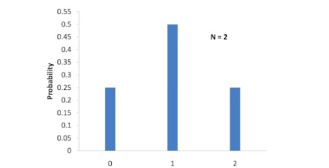
\includegraphics[width=0.5\textwidth]{images/0.png}
\caption{\label{fig:bin2}Binomial distribution of two event.}
\end{figure}

Then adding more event

\begin{figure}[H]
\centering
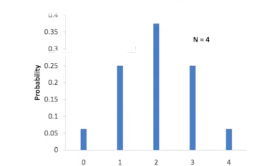
\includegraphics[width=0.5\textwidth]{images/1.png}
\caption{\label{fig:bin4}Binomial distribution of 4 event.}
\end{figure}
Then locking for a more crowded situation
\begin{figure}[H]
\centering
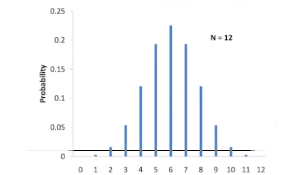
\includegraphics[width=0.5\textwidth]{images/2.png}
\caption{\label{fig:bin12}Binomial distribution of 12 event.}
\end{figure}

De Moivre understand the important of this result and try to find a way to write this curve
infact if you can replace the binomial coefficient graph that is made up of lots of bars by a smooth curve, then
instead of having to add lots of individual numbers you can just find the area under the curve, which is
exactly one of calculus’s strengths. You can see that as n increases the graphs look more and more like a
bell-curve.
DeMoivre began by considering the expansion of $ (1+1)^{n} $ . This expression comes up naturally in
analyzing a coin toss with equal probabilities of heads and tails. He focused on the ratio of the middle
term to the sum of all the coefficients, $ 2^n $ .
DeMoivre wanted to know what happens to the ratio when n gets very large. It is informative to see how a 17th century mathematician has to deal with such a problem.
He had “a dozen years or more” ago found that the ratio of the middle term to the sum can be expressed, using modern parentheses, as  $ R= 2A(n+1)^{n} / n^{n} \sqrt{n-1} $.

He wants to determine the value of R for any given n. Once he gets that, he knows the height of the curve at the middle and could then build the rest from that. He used some results he had found earlier about limits, some earlier work by James Bernoulli, and work that James Stirling did at just the right time to help.

First DeMoivre rewrites his fraction as   $ R= 2A/ \sqrt{n-1} * (1-(1/n))^{n} $.

Then since he wants to find the limiting value of this expression when n approaches infinity (Many mathematicians of that time were working on problems that involved expanding binomial expressions) he uses the earlier work by James Bernoulli to say that the limit for $ (1-(1/n))^{n} $ is “the number
whose hyperbolic logarithm is -1.” Today we say “natural” logarithm instead of hyperbolic logarithm,and we would therefore write $ \lim_{n\to\infty}  (1-(1/n))^{n}  = e^{-1}  $.
so for large value of n we car replace th limit with $ e^{-1} $
That gets us to the ratio as $ R=  \frac {2Ae^{-1}}{\sqrt(n-1)} $
He also states that he has shown in his own earlier work that A is the number whose hyperbolic logarithm is $ \frac{1}{12} - \frac{1}{360} + \frac{1}{1260} - \frac{1}{1680} + ...  $  or in modern notation $ e^{....} $
So doing some math we can rewrite R as $ \frac{2}{(e^{ \frac{1}{12} - \frac{1}{360} + \frac{1}{1260} - \frac{1}{1680} + ... }) \sqrt{n-1}  } $

DeMoivre called the messy looking part B. So he ends up with $ R= \frac{2}{B \sqrt{n-1}} $
DeMoivre says this is as far as had gotten when he had last worked on the problem.
It had been good enough for him to do some approximate calculations but he did not get a “nice” expression for B.
Lucky for him, his friend and colleague,
James Stirling, showed the exact value of B.
Since the circumference of a circle whose radius is 1 is $ \pi $, we can write DeMoivre’s formula for the desired ratio as R = $ \frac{2}{ \sqrt{2\pi}\sqrt{n-1} } $.
Then he reasoned that for really large values of n there’s no appreciable difference between $ \sqrt{n-1} $ and  $ \sqrt{n}$.
We can therefore write the ratio as  R = $ \frac{2}{ \sqrt{2\pi}\sqrt{n} } $.
This starts to look like the modern formula for the normal curve.
We can show the similarity further remembering that DeMoivre is approximating a binomial with $ p= \frac{1}{2} $. The standard deviation for a binomial distribution is given by $ \sigma = \sqrt{np(1-p)} $ and replaced p with $ \frac{1}{2} $  get us to $ \sigma = \frac{ \sqrt{n}}{2} $.
Solving this for $ \sqrt{n}$ we get $ \sqrt{n}= 2\sigma $.
And so finally R= $ \frac{1}{\sqrt{2\pi}\sigma}$
This is exactly the y value of the normal curve at the center where x = $ \mu $.
$ y= \frac{1}{\sqrt{2\pi}\sigma }e^{{\frac{-(x-\mu)^{2}}{2\sigma^{2}}}}=  \frac{1}{\sqrt{2\pi}\sigma} $

\subsubsection{Some statistical consequences of DeMoivre’s work on the normal curve.}
The formula itself would be found to have more and more applications, beyond just the approximation of a binomial distribution, especially as a model for the distribution of random measurement errors. Also,equally informative, the relationship $ \sigma = \frac{\sqrt{n}}{2}$, shows that the narrowness of the normal curve, as measured by $\sigma$, is proportional to the square-root of the sample size. This implies, for example, that if you wish to cut a margin of error in half, you will need four times as much information, not twice as much. Another way to say this is that the information you gain in collecting data is proportional, not to the number of pieces of data, but to its square root.

De Moivre’s approximations to binomial distributions did not do justice to the universality that characterizes the CLT. For the sake of completeness, but also to demonstrate what tremendous progress Laplace’s approximations of 1810 represented, de Moivre’s 1733 paper should be recognized as a sort of “0th chapter,” as it were, in the history of the CLT.



% The probability  distribution of many natural phenomenal are approximately a normal
\subsection{Gauss}
Gauss about 1800, used the normal distribution to describe the pattern of random
measurement error in observational data. Neither man used the name “normal curve.” That expression did not appear until the 1870s.
\section{The Central Limit Theorem from Laplace
to Cauchy: Changes in Stochastic Objectives
and in Analytical Methods}
in 1812, Pierre-Simon de Laplace (1749–1827) published the first edition of his
Théorie analytique des probabilités (henceforth simply abbreviated by TAP).1 With
its typical problems, stochastic models, and analytic methods this book would considerably influence probability theory and mathematical statistics right until the beginning of the 20th century.
Until Laplace and his successors, classical probability consisted mainly in the
sum of its applications to physical, social, and moral problems. However, as Laplace
already pointed out in the concise preface to the first edition of his TAP, probability
was also important for mathematics in a narrower sense. In many problems referring
to stochastic models depending on a large number of trials, probabilities could only
be expressed by formulae too complicated for direct numerical evaluation. Thus,
for a reasonable application of many of the results of probability calculus, particular considerations were needed to obtain useful approximations of the “formulae
of large numbers.” In the aforementioned preface, Laplace called these problems
“the most delicate, the most difficult, and the most useful” of the entire theory.
He expressed his hope that discussion of these problems would catch the attention of
other “geometers.” Therefore, in addition to the qualitative feature of applicability,
which was characteristic for classical probability theory, a new, purely mathematical
aspect emerged: the relevance of specific analytical methods of probability theory.
Laplace had been intensely dealing with the “delicate problems” of probability
just described from the very beginning of his scientific career. In his 1781 “Mémoire
sur les probabilités,” one can already find “in nuce” almost all of the problems of
TAP, which can be roughly divided into two categories: “sums of random variables”
and “inverse probabilities.”2 The first category includes, for example, the a priori
probabilities of profit and loss in certain games of chance, or of the arithmetic mean
of observations being subject to random errors; the latter for instance deals with the
a posteriori probabilities that the ratio of the chances of a boy’s and a girl’s birth
is within a given interval centered around the ratio of the corresponding observed
values. By 1774, Laplace had already developed useful approximation methods for
those a posteriori probabilities depending on a large number of observations. He did
not succeed in adapting this method to a priori probabilities until 1810, however.
Only then, with a “tricky” modification of the method of generating functions, did
he achieve any usable results on approximations of probabilities of sums of independent random variables, which, from the modern point of view, are subsumed under
the rubric of the “central limit theorem.” It was the CLT which considerably shaped
the contents and methods of the TAP and significantly influenced the development
of probability and error theory during the 19th century.
As we have already seen (Sect. 1.4), the history of the CLT, as far as the contributions of Laplace and his successors are concerned, has already been studied in
fair detail. Therefore, a main focus in the present section will be on those questions
which still seem to be open: Which changes in the probabilistic and analytical context of the CLT occurred between ca. 1810 and 1850; how did these changes come
about, and how have these changes influenced analytical style and methods in the
treatment of this theorem?
\subsection{Laplace’s Central “Limit” Theorem}
As already noticed, Laplace’s CLT was the result of an almost forty years’ effort.
In the following, we will describe the historical development of Laplace’s treatment
of sums of independent random variables, his methods for finding appropriate approximation formulae, and the major applications of his finally achieved CLT.
\subsubsection{Sums of Independent Random Variables}
Sums of independent random variables had played an important role in Laplace’s
probabilistic work from the very beginning.3 In this context, the problem of calculating the probability distribution of the sum of angles of inclination, which were
assumed to be determined randomly, as well as the related problem of calculating
the probabilities of the deviations between the arithmetic mean of data which were
afflicted by observational errors and the underlying “true value,” became especially
important. In one of his first published papers, Laplace [1776] had already set out to
determine the probability that the sum of the angles of inclination of comet orbits (or
the arithmetic mean of these angles respectively) is within given limits. He assumed
that all angles, which had to be measured against the ecliptic, were distributed randomly according to a uniform distribution between 0ı and 90ı (and also tacitly
presupposed that all angles were stochastically independent). Laplace succeeded in
calculating these probabilities for an arbitrary number of comets via induction (with
a minor mistake which was subsequently corrected in [Laplace 1781]). In this 1781
paper, Laplace even introduced a general—however very intricate—method, based
on convolutions of density functions, in order to exactly determine the probability
that a sum of independent random variables (“quantités variables,” as Laplace put it)
was within given limits.In the most simple case, each of the n variables had the
same rectangular distribution between 0 and h. For the probability P that the sum
of those variables was between a and b with $ 0 \leq a< b \leq nh $ , Laplace obtained (in
modern notation)

$ P= \frac{1}{h^{n}n!}(\sum\limits_{n=0}^{N}\binom{n}{i}(-1)^{i}(b-ih)^{n}- \sum\limits_{i=0}^{M}\binom{n}{i}(-1)^{i}(a-ih)^{n}  ) $

where $ N= \min(n,[\frac{b}{h}]) $ and $ M= \min(n,[\frac{a}{h}])$.
Formulae of this kind were too complicated for a direct numerical evaluation if the number of random variables exceeded a relatively small value. The arithmetic mean of the actual observed angles of inclination of the then known 63 comets was $46^{\circ} 16^{\prime} $. Through the use of
upper formula  alone, Laplace was unable to address the hypothesis that the comets’ planes
of motion resulted at “random.” At this stage of his mathematical work, however,Laplace could not develop usable approximation.

\subsection{Prove}
The standard version of the central limit theorem was first proved by the French mathematician Pierre-Simon Laplace in 1810, states that the sum or average of an infinite sequence of independent and identically distributed random variables, when suitably rescaled, tends to a normal distribution.
Fourteen years later the French mathematician Siméon-Denis Poisson began a continuing process of improvement and generalization.
Laplace and his contemporaries were interested in the theorem primarily because of its importance in repeated measurements of the same quantity. If the individual measurements could be viewed as approximately independent and identically distributed, then their mean could be approximated by a normal distribution.







\subsection{How to create Sections and Subsections}

  Simply use the section and subsection commands, as in this example document! With Overleaf, all the formatting and numbering is handled automatically according to the template you've chosen. If you're using Rich Text mode, you can also create new section and subsections via the buttons in the editor toolbar.

\subsection{How to include Figures}

First you have to upload the image file from your computer using the upload link in the file-tree menu. Then use the includegraphics command to include it in your document. Use the figure environment and the caption command to add a number and a caption to your figure. See the code for Figure \ref{fig:frog} in this section for an example.

Note that your figure will automatically be placed in the most appropriate place for it, given the surrounding text and taking into account other figures or tables that may be close by. You can find out more about adding images to your documents in this help article on \href{https://www.overleaf.com/learn/how-to/Including_images_on_Overleaf}{including images on Overleaf}.

\begin{figure}[H]
\centering

\includegraphics[width=0.3\textwidth]{images/frog.jpg}
\caption{\label{fig:frog}This frog was uploaded via the file-tree menu.}
\end{figure}

\subsection{How to add Tables}

Use the table and tabular environments for basic tables --- see Table~\ref{tab:widgets}, for example. For more information, please see this help article on \href{https://www.overleaf.com/learn/latex/tables}{tables}.

\begin{table}[H]
\centering
\begin{tabular}{l|r}
Item & Quantity \\\hline
Widgets & 42 \\
Gadgets & 13
\end{tabular}
\caption{\label{tab:widgets}An example table.}
\end{table}

\subsection{How to add Comments and Track Changes}

Comments can be added to your project by highlighting some text and clicking ``Add comment'' in the top right of the editor pane. To view existing comments, click on the Review menu in the toolbar above. To reply to a comment, click on the Reply button in the lower right corner of the comment. You can close the Review pane by clicking its name on the toolbar when you're done reviewing for the time being.

Track changes are available on all our \href{https://www.overleaf.com/user/subscription/plans}{premium plans}, and can be toggled on or off using the option at the top of the Review pane. Track changes allow you to keep track of every change made to the document, along with the person making the change.

\subsection{How to add Lists}

You can make lists with automatic numbering \dots

\begin{enumerate}
\item Like this,
\item and like this.
\end{enumerate}
\dots or bullet points \dots
\begin{itemize}
\item Like this,
\item and like this.
\end{itemize}

\subsection{How to write Mathematics}

\LaTeX{} is great at typesetting mathematics. Let $X_1, X_2, \ldots, X_n$ be a sequence of independent and identically distributed random variables with $\text{E}[X_i] = \mu$ and $\text{Var}[X_i] = \sigma^2 < \infty$, and let
\[S_n = \frac{X_1 + X_2 + \cdots + X_n}{n}
      = \frac{1}{n}\sum_{i}^{n} X_i\]
denote their mean. Then as $n$ approaches infinity, the random variables $\sqrt{n}(S_n - \mu)$ converge in distribution to a normal $\mathcal{N}(0, \sigma^2)$.


\subsection{How to change the margins and paper size}

Usually the template you're using will have the page margins and paper size set correctly for that use-case. For example, if you're using a journal article template provided by the journal publisher, that template will be formatted according to their requirements. In these cases, it's best not to alter the margins directly.

If however you're using a more general template, such as this one, and would like to alter the margins, a common way to do so is via the geometry package. You can find the geometry package loaded in the preamble at the top of this example file, and if you'd like to learn more about how to adjust the settings, please visit this help article on \href{https://www.overleaf.com/learn/latex/page_size_and_margins}{page size and margins}.

\subsection{How to change the document language and spell check settings}

Overleaf supports many different languages, including multiple different languages within one document.

To configure the document language, simply edit the option provided to the babel package in the preamble at the top of this example project. To learn more about the different options, please visit this help article on \href{https://www.overleaf.com/learn/latex/International_language_support}{international language support}.

To change the spell check language, simply open the Overleaf menu at the top left of the editor window, scroll down to the spell check setting, and adjust accordingly.

\subsection{How to add Citations and a References List}

You can simply upload a \verb|.bib| file containing your BibTeX entries, created with a tool such as JabRef. You can then cite entries from it, like this: \cite{greenwade93}. Just remember to specify a bibliography style, as well as the filename of the \verb|.bib|. You can find a \href{https://www.overleaf.com/help/97-how-to-include-a-bibliography-using-bibtex}{video tutorial here} to learn more about BibTeX.

If you have an \href{https://www.overleaf.com/user/subscription/plans}{upgraded account}, you can also import your Mendeley or Zotero library directly as a \verb|.bib| file, via the upload menu in the file-tree.

\subsection{Good luck!}

We hope you find Overleaf useful, and do take a look at our \href{https://www.overleaf.com/learn}{help library} for more tutorials and user guides! Please also let us know if you have any feedback using the Contact Us link at the bottom of the Overleaf menu --- or use the contact form at \url{https://www.overleaf.com/contact}.

\bibliographystyle{alpha}
\bibliography{statistics}


\end{document}
